\documentclass{article}
\usepackage{amsmath}
\usepackage{amsthm}
\usepackage{amssymb}
\usepackage{enumerate}
\usepackage{graphicx}
% done
\begin{document}
    \title{MA4\_2 Exercise}
    \author{Wang Yue from CS Elite Class}
    \date{\today}

    \maketitle

    \section*{Exercise 4.4}

    
    \subsection*{20. $\lim_{x \to \infty}\frac{\ln \ln x}{x}$}

    $$\begin{aligned}
        \lim_{x \to \infty}\frac{\ln \ln x}{x} &= \lim_{x \to \infty}\frac{\frac{1}{x\ln x}}{1} \\
        &= \frac{1}{x \ln x} \\
        &= 0
    \end{aligned}$$

    \subsection*{23. $\lim_{x \to 0}\frac{\sqrt{1 + 2x} - \sqrt{1 - 4x}}{x}$}

    $$\begin{aligned}
        \lim_{x \to 0}\frac{\sqrt{1 + 2x} - \sqrt{1 - 4x}}{x} &= \lim_{x \to 0}\frac{1 + 2x - (1 - 4x)}{x(\sqrt{1 + 2x} + \sqrt{1 + 4x})} \\
        &= \lim_{x\to 0} \frac{6}{\sqrt{1 + 2x} + \sqrt{1 - 4x}} \\
        &= \frac{6}{1 + 1} \\
        &= 3
    \end{aligned}$$

    \subsection*{25. $\lim_{x \to 0}\frac{e^x - 1 - x}{x^2}$}

    $$\begin{aligned}
        \lim_{x \to 0}\frac{e^x - 1 - x}{x^2} &= \lim_{x \to 0}\frac{e^x - 1}{2x} \\
        &= \lim_{x \to 0}\frac{e^x}{2} \\
        &= \frac 1 2
    \end{aligned}$$

    \subsection*{35. $\lim_{x \to 1}\frac{1 - x + \ln x}{1 + \cos \pi x}$}

    $$\begin{aligned}
        \lim_{x \to 1}\frac{1 - x + \ln x}{1 + \cos \pi x} &= \lim_{x \to 1}\frac{-1 + \frac 1 x}{-\pi \sin \pi x} \\
        &= \lim_{x \to 1}\frac{x - 1}{\pi x \sin \pi x} \\
        &= \lim_{x \to 1}\frac{1}{\pi(\sin \pi x + \pi x \cos \pi x)} \\
        &= \frac{1}{-\pi ^2}
    \end{aligned}$$

    \subsection*{44. $\lim_{x \to 0^+}(\sin x \ln x)$}

    $$\begin{aligned}
        \lim_{x \to 0^+}\sin \ln x &= \lim_{x \to 0^+}\frac{\ln x}{\frac{1}{\sin x}} \\
        &= \lim_{x \to 0^+}\frac{\frac 1 x}{\frac{- \cos x}{\sin ^2 x}} \\
        &= \lim_{x \to 0^+}\frac{-\tan x}{x \cos x} \\
        &= \lim_{x \to 0^+}\frac{-x}{x \cos x} \\
        &= \lim_{x \to 0^+}\frac{-1}{\cos x} = -1
    \end{aligned}$$

    \subsection*{49. $\lim_{x \to 1}(\frac{x}{x - 1} - \frac{1}{\ln x})$}

    $$\begin{aligned}
        \lim_{x \to 1}(\frac{x}{x - 1} - \frac{1}{\ln x}) &= \lim_{x \to 1}\frac{x\ln x - x + 1}{(x - 1)\ln x} \\
        &= \lim_{x \to 1}\frac{\ln x + 1 - 1}{\ln x + \frac{x - 1}{x}} \\
        &= \lim_{x \to 1}\frac{\ln x}{\ln x + 1 - \frac 1 x} \\
        &= \lim_{x \to 1}\frac{\frac 1 x}{\frac 1 x + \frac{1}{x^2}} \\
        &= \lim_{x \to 1}\frac{x}{x + 1} \\
        &= \frac 1 2
    \end{aligned}$$

    \subsection*{52. $\lim_{x \to 0^+}(\cot x - \frac 1 x)$}

    $$\begin{aligned}
        \lim_{x \to 0^+}(\cot x - \frac 1 x) &= \lim_{x \to 0^+}(\frac{\cos x}{\sin x} - \frac 1 x) \\
        &= \lim_{x \to 0^+}\frac{x \cos x - \sin x}{x \sin x} \\
        &= \lim_{x\ to 0^+}\frac{\cos x - x \sin x - \cos x}{\sin x + x \cos x} \\
        &= \lim_{x \to 0^+}\frac{-\sin x}{\frac{\sin x}{x} + \cos x} \\
        &= \lim_{x \to 0^+}\frac{-\sin x}{1 + \cos x} \\
        &= 0
    \end{aligned}$$

    \subsection*{55. $\lim_{x \to 0^+}x^{\sqrt x}$}
    
        $$\lim_{x \to 0^+}x^{\sqrt x} = \lim_{x \to 0^+}e^{\sqrt{x} \ln x} $$
    $$\begin{aligned}
        \because \lim_{x \to 0^+} \sqrt{x} \ln x &= \lim_{x \to 0^+}\frac{\ln x}{x^{-\frac 1 2}} \\
        &= \lim_{x \to 0^+}-2\sqrt{x} \\
        &= 0
    \end{aligned}$$

    $$\therefore \lim_{x \to 0^+}\sqrt x \ln x = e^0 = 1$$

    \subsection*{58. $\lim_{x \to \infty}(1 + \frac a x)^{bx}$}

    $$\lim_{x \to \infty}(1 + \frac a x)^{bx} = \lim_{x \to \infty} e^{ bx \ln (1 + \frac a x)} $$

    $$\begin{aligned}
        \because \lim_{x \to \infty}bx \ln (1 + \frac a x) &= \lim_{x \to \infty}\frac{\ln (1 + \frac a x)}{\frac{1}{bx}} \\
        &= \lim_{x \to \infty}\frac{\frac{-\frac{a}{x^2}}{1 + \frac a x}}{-\frac{1}{bx^2}} \\
        &= \lim_{x \to \infty}\frac{ab}{1 + \frac a x} \\
        &= \frac{ab}{1 + 0} = ab
    \end{aligned}$$

    $$\therefore \lim_{x \to \infty}(1 + \frac a x)^{bx} = e^{ab}$$

    \subsection*{62. $\lim_{x\to \infty}(e^x + x)^{\frac 1 x}$}

    $$\lim_{x \to \infty}(e^x + x)^{\frac 1 x} = \lim_{x \to \infty}e^{\frac 1 x \ln(e^x + x)}$$
    $$\begin{aligned}
        \because \lim_{x \to \infty}\frac{\ln(e^x + x)}{x} &= \lim_{x \to \infty}\frac{\frac{e^x + 1}{e^x + x}}{1} \\
        &= \lim_{x \to \infty}\frac{e^x}{e^x + 1} \\
        &= \lim_{x \to \infty}(1 - \frac{1}{e^x  + 1}) \\
        &= 1
    \end{aligned}$$

    $$\therefore \lim_{x \to \infty}(e^x + x) ^{\frac 1 x} = e^1 = e$$

    \subsection*{66. $\lim_{x \to \infty}(\frac{2x - 3}{2x + 5})^{2x + 1}$}

    $$\lim_{x \to \infty}(\frac{2x - 3}{2x + 5})^{2x + 1} = \lim_{x \to \infty}e^{(2x + 1) \ln \frac{2x - 3}{2x + 5}}$$

    $$\begin{aligned}
        \lim_{x \to \infty}(2x + 1)\ln \frac{2x - 3}{2x + 5} &= \lim_{x \to \infty}\frac{\ln \frac{2x - 3}{2x + 5}}{\frac{1}{2x + 1}} \\
        &= \lim_{x \to \infty}\frac{\frac{2x + 5}{2x - 3} \frac{2(2x + 5) - 2(2x + 3)}{(2x + 5)^2}}{\frac{-2}{(2x + 1)^2}} \\
        &= \lim_{x \to \infty}\frac{-2(2x + 1)^2}{(2x - 3)(2x + 5)} \\
        &= \lim_{x \to \infty}\frac{-2 \times 2(2x + 1) \times 2}{2(2x + 5) + 2(2x - 3)} \\
        &= \lim_{x \to \infty}\frac{-8(2x + 1)}{2(2x + 1)} \\
        &= -4
    \end{aligned}$$

    $$\therefore \lim_{x \to \infty}(\frac{2x - 3}{2x + 5})^{2x + 1} = e^{-4}$$

    \subsection*{87. If $f'$ is continuous, use l'Hospital's Rule to show that $$\lim_{h \to 0}\frac{f(x + h) - f(x - h)}{2h} = f'(x)$$ Explain the meaning of this equation with the aid of a diagram.}

    Use l'Hospital Rule with respect to $h$, and we get

    $$\begin{aligned}
        \lim_{h \to 0}\frac{f(x + h) - f(x - h)}{2h} &= \lim_{h \to 0}\frac{f'(x + h) + f'(x - h)}{2} \\
        &= f'(x)
    \end{aligned}$$

    The meaning of this equation is the slope of the tangent line to $f$.

    The following diagram describes the situation as $f(x) = x^2, x = 1, h = 0.05$.

    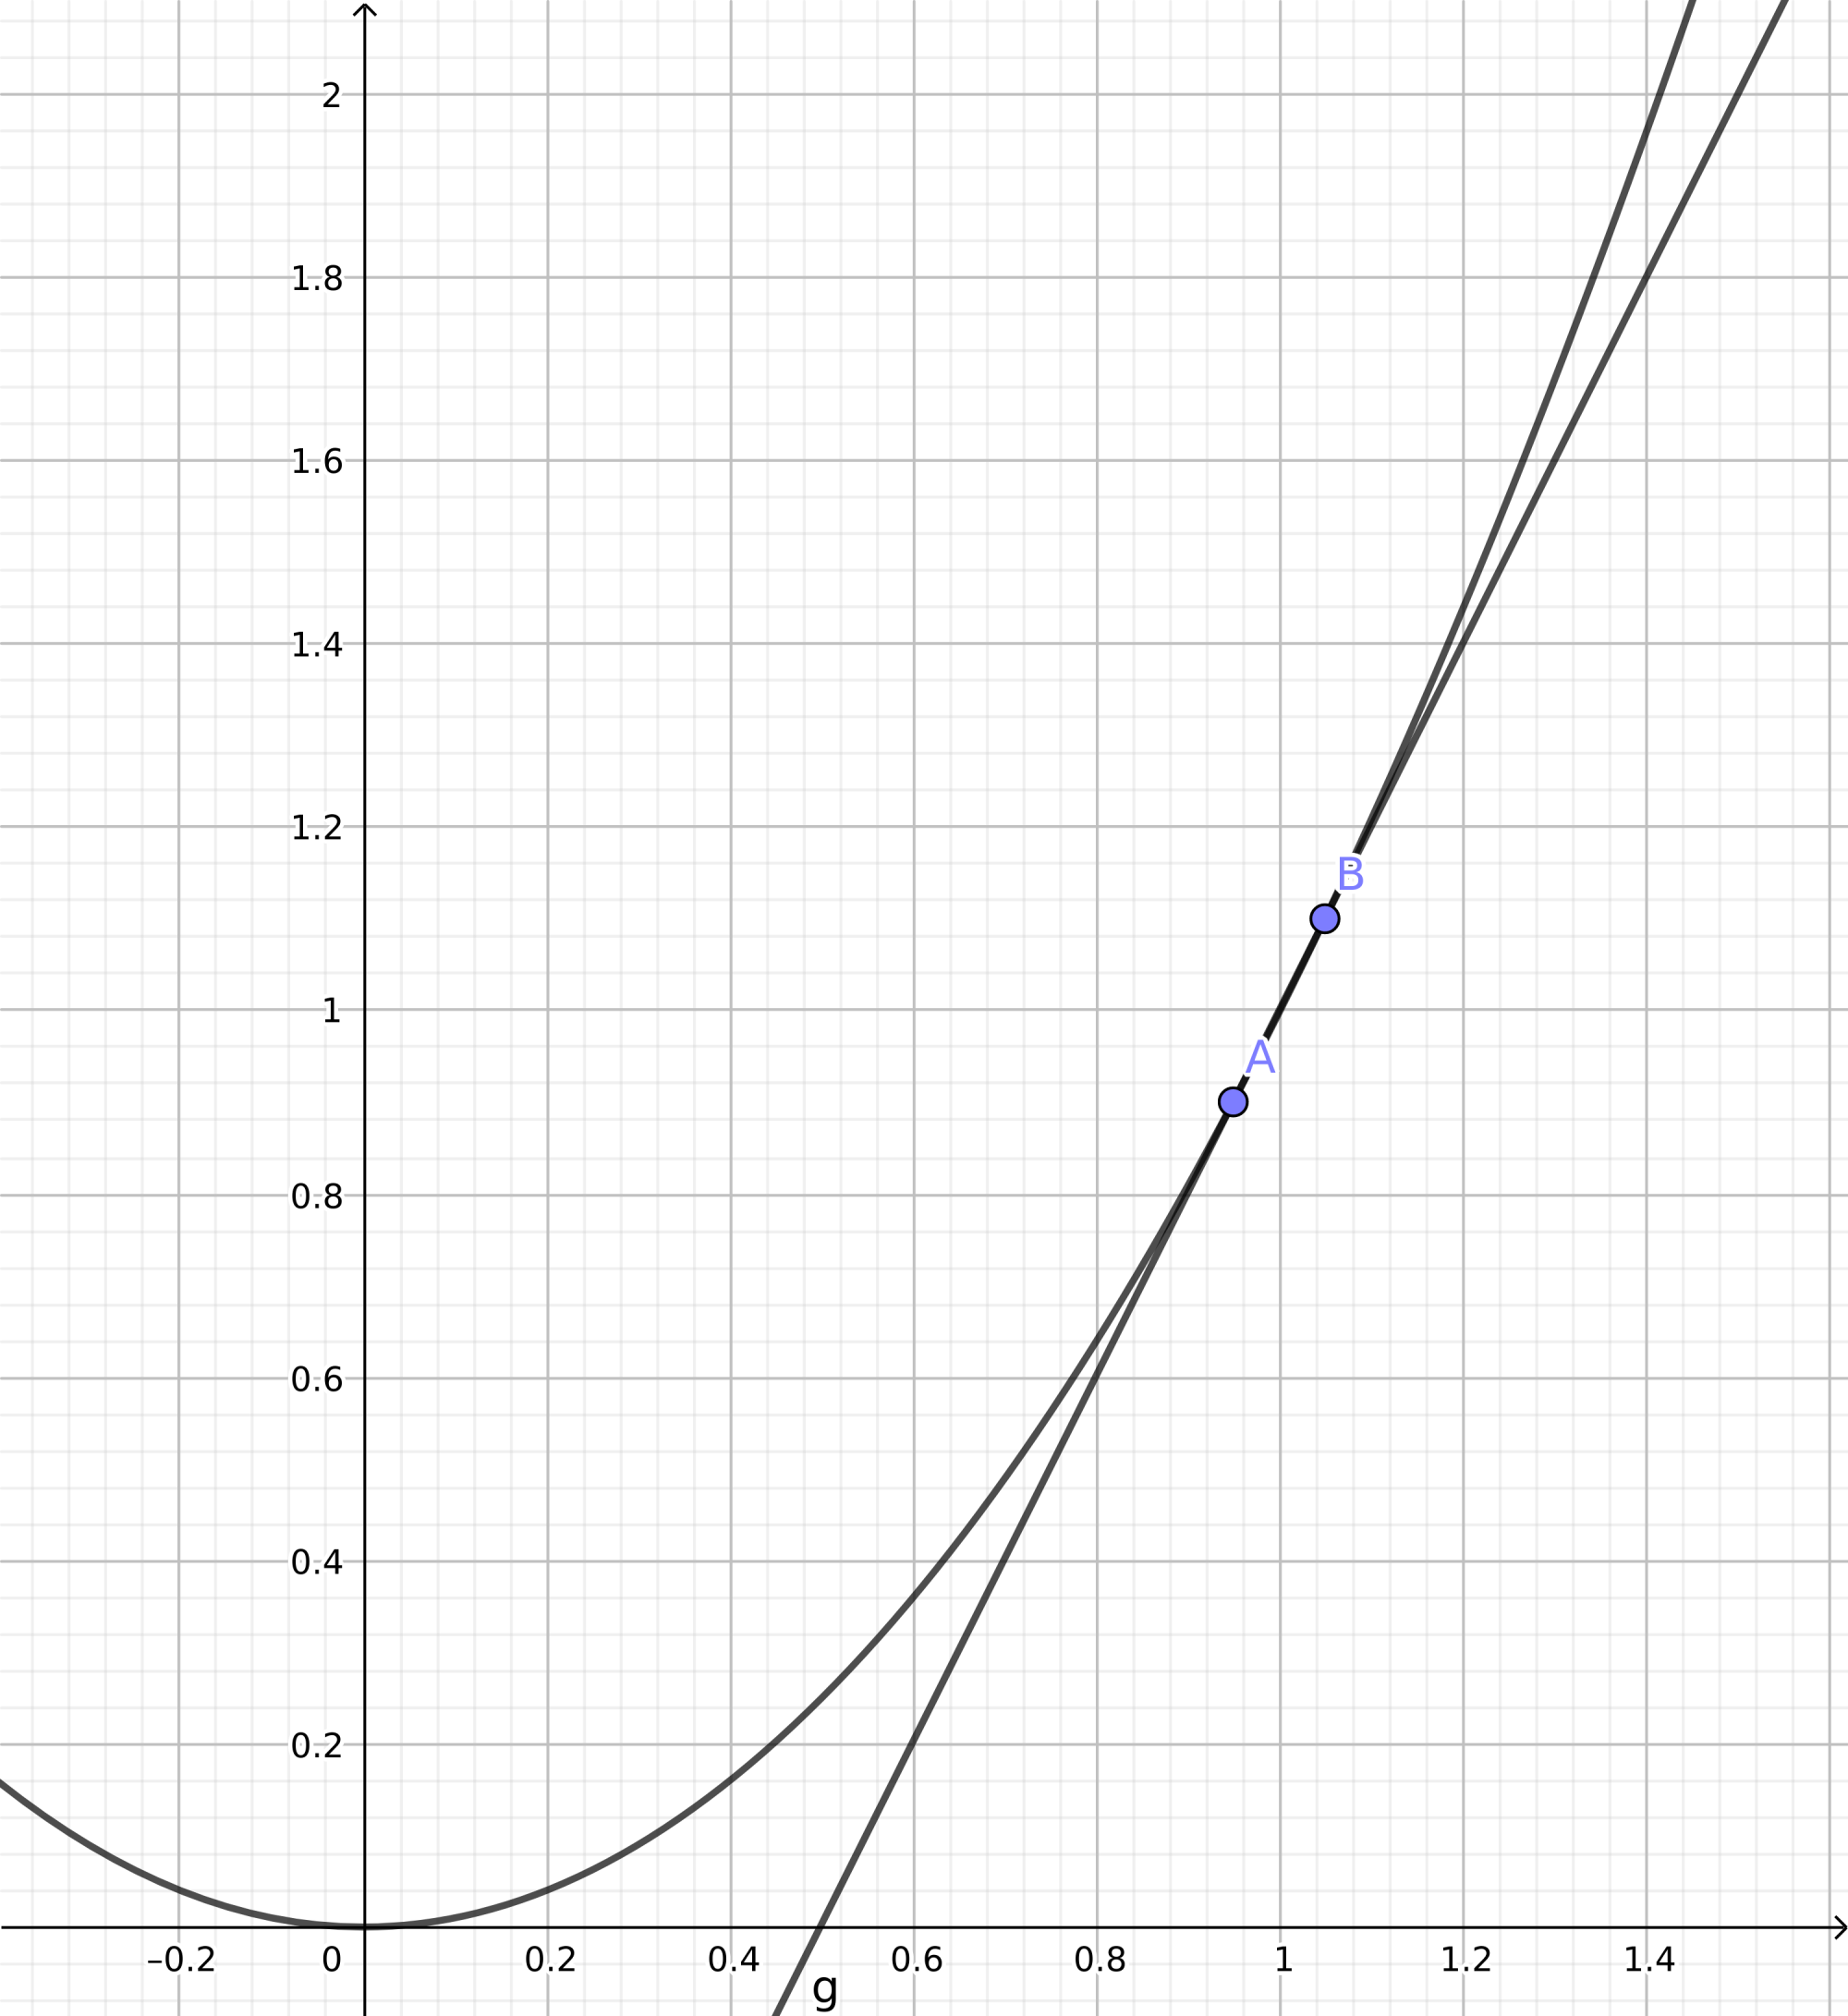
\includegraphics[scale=6]{87.png}

    \subsection*{88. If $f''$ is continuous, show that $$\lim_{h \to 0}\frac{f(x + h) - 2f(x) + f(x - h)}{h^2} = f''(x)$$}

    $$\begin{aligned}
        \lim_{h \to 0}\frac{f(x + h) - 2f(x) + f(x - h)}{h^2} &= \lim_{h \to 0}\frac{f'(x + h) - f'(x - h)}{2h} \\
        &= \lim_{h \to 0}\frac{f'(x + h) - f'(x) + f'(x) - f'(x - h)}{2h} \\
        &= \lim_{h \to 0}\frac 1 2(\frac{f'(x + h) - f'(x)}{h} + \frac{f'(x) - f'(x - h)}{h}) \\
        &= \frac{2f''(x)}{2} = f''(x)
    \end{aligned}$$

    \subsection*{89. Let $$f(x) = \left\{ \begin{array}{ll}
        e^{-\frac{1}{x^2}} & \textrm{if $x \not = 0$} \\
        0 & \textrm{if $x = 0$} \end{array} \right . $$}
    \begin{enumerate}[(a)]
        \item Use the definition of derivative to compute $f'(0)$.

        $$\begin{aligned}
            f'(0) &= \lim_{x \to 0}\frac{f(x) - f(0)}{x - 0} \\
            &= \lim_{x \to 0}\frac{e^{-x^{-2}}}{x} \\
            &= \lim_{x \to 0}\frac{\frac{1}{x}}{e^{x^{-2}}} \\
            &= \lim_{x \to 0}\frac{-\frac{1}{x^2}}{-2e^{x^{-2}}x^{-3}} \\
            &= \lim_{x \to 0}\frac{x}{2e^{x^{-2}}} \\
            &= 0
        \end{aligned}$$

        \item Show that $f$ has derivatives of all orders that are defined on $R$.

        \begin{proof}
            Suppose $$f^{(n)}(x) = \left\{ \begin{array}{ll}
                0 & \textrm{if $x = 0$} \\
                y(n)e^{-x^{-2}} & \textrm{if $x \not = 0$}
            \end{array} \right.$$

            in which $y(n)$ is a polymonial with respect to $x$.

            We will prove it by mathematical induction.

            $4e^{-x^{-2}}x^{-3} - 6e^{-x^{-2}}x^{-4} = e^{-x^{-2}}(4x^{-3} - 6x^{-4})$

            When $n = 1$, $$f^{(1)}(x) = \left\{ \begin{array}{ll}
                0 & \textrm{if $x = 0$} \\
                2e^{-x^{-2}}x^{-3} & \textrm{if $x \not = 0$}
            \end{array} \right.$$ which means that when $n = 1$, $y(1) = x^{-3}$, $f^{(n)}(x)$ exists for all $x \in R$.

            When $n \geq 2$, suppose that $f^{(n)}(x)$ exists when $n = k, k \in N_+$.

            If $x = 0$, $$f^{(k + 1)}(x) = (f^{(k)}(x))' = (0)' = 0$$

            If $x \not = 0$, $$\begin{aligned}
                f^{(k + 1)}(x) &= (f^{(k)}(x))' \\
                &= (y(k)e^{-x^{-2}})' \\
                &= (y'(k) + 2x^{-3})e^{-x^{-2}} \\
                &= y(k + 1)e^{-x^{-2}}
            \end{aligned}$$

            Since $y(k + 1)$ is a polymonial, $y(k + 1)e^{-x^{-2}}$ can be defined when $x \not = 0$.

            Therefore $f^{(k + 1)}(x)$ can be defined on $R$.

            In all, $f^{(n)}(x)$ can be defined on $R$.


        \end{proof}

    \end{enumerate}
    % 20 23 25 35 44 49 52 55 58 62 66 87 88 89
\end{document}